\section{Evaluation}
\FloatBarrier%
The results of all three models tested with the basic parameters
(\cref{tbl:params}) on various input sizes is shown in \cref{fig:result}. At
very low training sizes, the F1 scores are about the same, with a very high
variance. At higher training sizes, the \texttt{Clusters} model pulls ahead with
a small, but statistically significant lead over the baseline
(see \cref{tbl:base_cl} for the raw numbers). The \texttt{Clusters-LSTM} model
performs similarly to the \texttt{Clusters} models, only scoring higher in a
barely significant way at 400 samples. 

\begin{figure}[tb]
  \centering
  %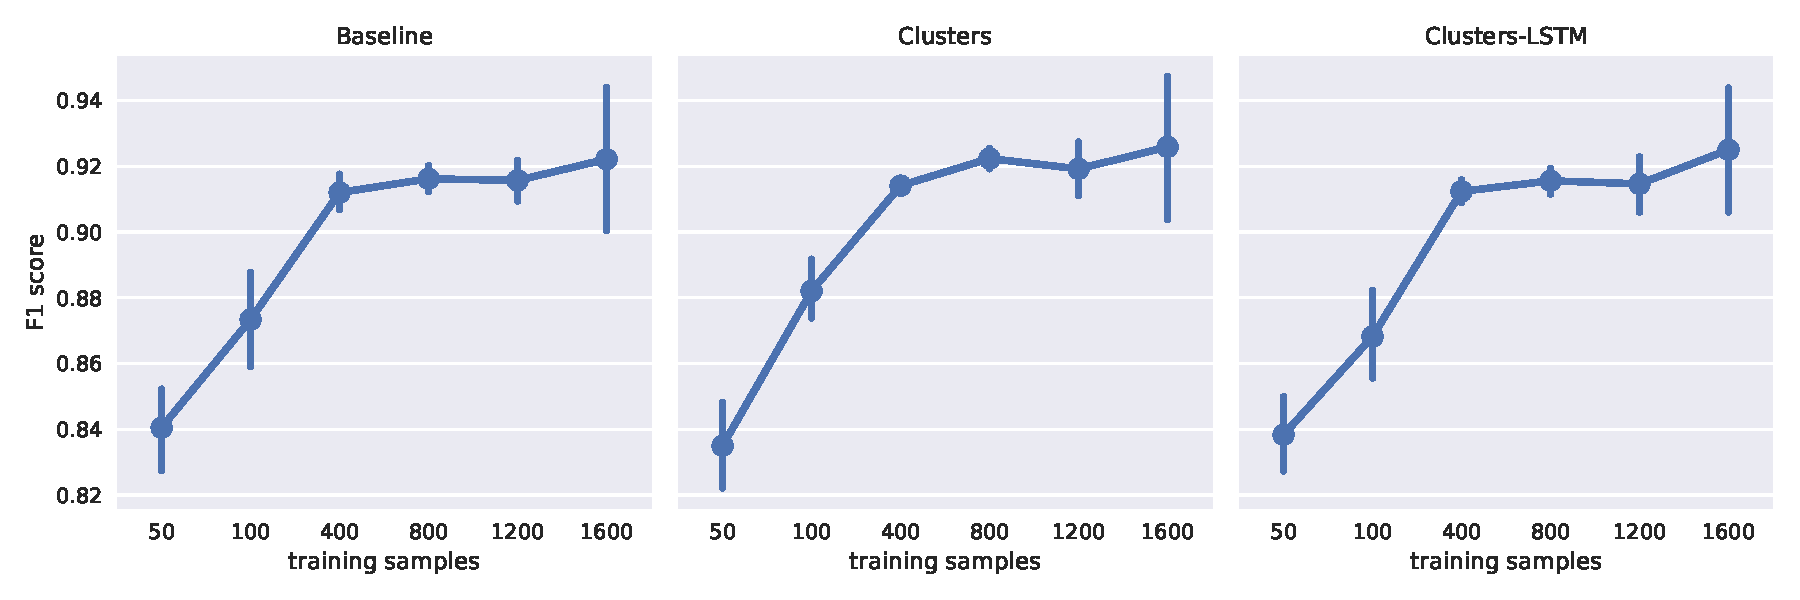
\includegraphics[width=\textwidth]{figures/results/main/factorplot_f1.pdf}
  \caption{This figure compares the performance of the baseline model, using
    only a CNN, to that of the model augmented with clustering. The vertical axis
    shows the F1 score, averaged over 10 trials. The horizontal axis shows the
    number of samples used for training (at a 1:1 ratio of positive to negative
    samples). The vertical bars indicate confidence intervals, meaning that based on
    the observed F1 scores and assuming normality, the true mean is 95\% likely to
  fall within the shown interval.\label{fig:result}}
\end{figure}
\begin{table}[tb]
  \centering
  \begin{tabular}{lrrrr}
    \toprule
    \multirow{2}[3]{*}{\# training samples} & \multicolumn{2}{c}{F1 score} & \multirow{2}[3]{*}{p} \\
    \cmidrule(lr){2-3}
    & \multicolumn{1}{c}{Baseline} & \multicolumn{1}{c}{Clusters} & \\
    \midrule
    50   & 0.830 (\emph{0.035}) & 0.839 (\emph{0.026}) & 0.40 \\
    100  & 0.869 (\emph{0.025}) & 0.880 (\emph{0.017}) & 0.19 \\
    400  & 0.903 (\emph{0.007}) & 0.910 (\emph{0.006}) & \textbf{0.005} \\
    800  & 0.911 (\emph{0.008}) & 0.914 (\emph{0.007}) & 0.15 \\
    1200 & 0.911 (\emph{0.011}) & 0.919 (\emph{0.011}) & \textbf{0.008} \\
    \bottomrule
  \end{tabular}
  \caption{The values corresponding to \cref{fig:result}, comparing the
    \texttt{Baseline} and \texttt{Clusters} model. The final column shows
    that probability of the F1 scores of both models being drawn from the same
  distribution.\label{tbl:base_cl}}
\end{table}
\begin{table}[tb]
  \centering
  \begin{tabular}{lrrrr}
    \toprule
    \multirow{2}[3]{*}{\# training samples} & \multicolumn{2}{c}{F1 score} & \multirow{2}[3]{*}{p} \\
    \cmidrule(lr){2-3}
    & \multicolumn{1}{c}{Clusters} & \multicolumn{1}{c}{Clusters-LSTM} & \\
    \midrule
    50   & 0.839 (\emph{0.035}) & 0.820 (\emph{0.025}) & 0.43 \\
    100  & 0.880 (\emph{0.017}) & 0.877 (\emph{0.022}) & 0.72 \\
    400  & 0.910 (\emph{0.006}) & 0.913 (\emph{0.008}) & \textbf{0.027} \\
    800  & 0.914 (\emph{0.007}) & 0.919 (\emph{0.005}) & 0.11 \\
    1200 & 0.919 (\emph{0.011}) & 0.921 (\emph{0.005}) & 0.62 \\
    \bottomrule
  \end{tabular}
  \caption{The values corresponding to \cref{fig:result}, comparing the
    \texttt{Clusters} and \texttt{Clusters-LSTM} model. The final column shows
    that probability of the F1 scores of both models being drawn from the same
  distribution.\label{tbl:cl_cllstm}}
\end{table}

%%% Local Variables:
%%% mode: latex
%%% TeX-master: "report"
%%% End:
